\subsection{Nixtla NeuralForecast}
{{\footnotesize
\noindent NeuralForecast offers scalable, user-friendly implementations of over 30 neural forecasting models (NBEATS, NHITS, TFT, DeepAR, etc.),
emphasizing quality, usability, interpretability, and performance.


\begin{description}[labelwidth=4cm, labelsep=1em, leftmargin=4cm, itemsep=0.1em, parsep=0em]
  \item[date:] 2022-04-01
  \item[version:] v3.0.2
  \item[last\_updated:] 2025-06
  \item[expired:] unknown
  \item[valid:] yes
  \item[valid\_date:] 2022-04-01
  \item[url:] \href{https://github.com/Nixtla/neuralforecast}{https://github.com/Nixtla/neuralforecast}
  \item[doi:] unknown
  \item[domain:] Time-series forecasting; General ML
  \item[focus:] High-performance neural forecasting library with >30 models
  \item[keywords:]
    - time-series
    - neural forecasting
    - NBEATS, NHITS, TFT
    - probabilistic forecasting
    - usability
  \item[licensing:] Apache License 2.0
  \item[task\_types:]
    - Time-series forecasting
  \item[ai\_capability\_measured:]
    - Forecast accuracy
    - interpretability
    - speed
  \item[metrics:]
    - RMSE
    - MAPE
    - CRPS
  \item[models:]
    - NBEATS
    - NHITS
    - TFT
    - DeepAR
  \item[ml\_motif:]
    - Time-series
  \item[type:] Platform
  \item[ml\_task:]
    - Forecasting
  \item[solutions:] 0
  \item[notes:] AutoModel supports hyperparameter tuning and distributed execution via Ray and Optuna. First official NHITS implementation. contentReference oaicite:4 ndex=4

  \item[contact.name:] Kin G. Olivares (Nixtla)
  \item[contact.email:] unknown
  \item[results.links.name:] ChatGPT LLM
  \item[fair.reproducible:] Yes
  \item[fair.benchmark\_ready:] Yes
  \item[id:] nixtla\_neuralforecast
  \item[Citations:] \cite{olivares2022library_neuralforecast}
\end{description}

{\bf Ratings:} ~ \\

\begin{tabular}{p{0.15\textwidth} p{0.07\textwidth} p{0.7\textwidth}}
\hline
Rating & Value & Reason \\
\hline
dataset & 3 & NeuralForecast does not include its own datasets but supports standard datasets (e.g., M4, M5, ETT).
FAIR compliance depends on user-supplied data.
 \\
documentation & 5 & Rich documentation with examples, API references, tutorials, notebooks, and CLI support.
PyPI, GitHub, and official blog posts offer clear guidance for usage and extension.
 \\
metrics & 5 & RMSE, MAPE, CRPS, and other domain-relevant metrics are well supported and integrated into the evaluation loop.
 \\
reference\_solution & 4 & Includes runnable model baselines and training scripts for all supported models.
Some models have pretrained weights, but not all are fully benchmarked out-of-the-box.
 \\
software & 5 & Actively maintained open-source library under Apache 2.0. Offers a clean API,
extensive model zoo (>30 models), integration with Ray, Optuna, and supports
scalable training and inference workflows.
 \\
specification & 5 & Forecasting task is well-defined with clear input/output structures. Framework supports
probabilistic and deterministic forecasting, with unified interfaces and support for batch evaluation.
 \\
\hline
\end{tabular}

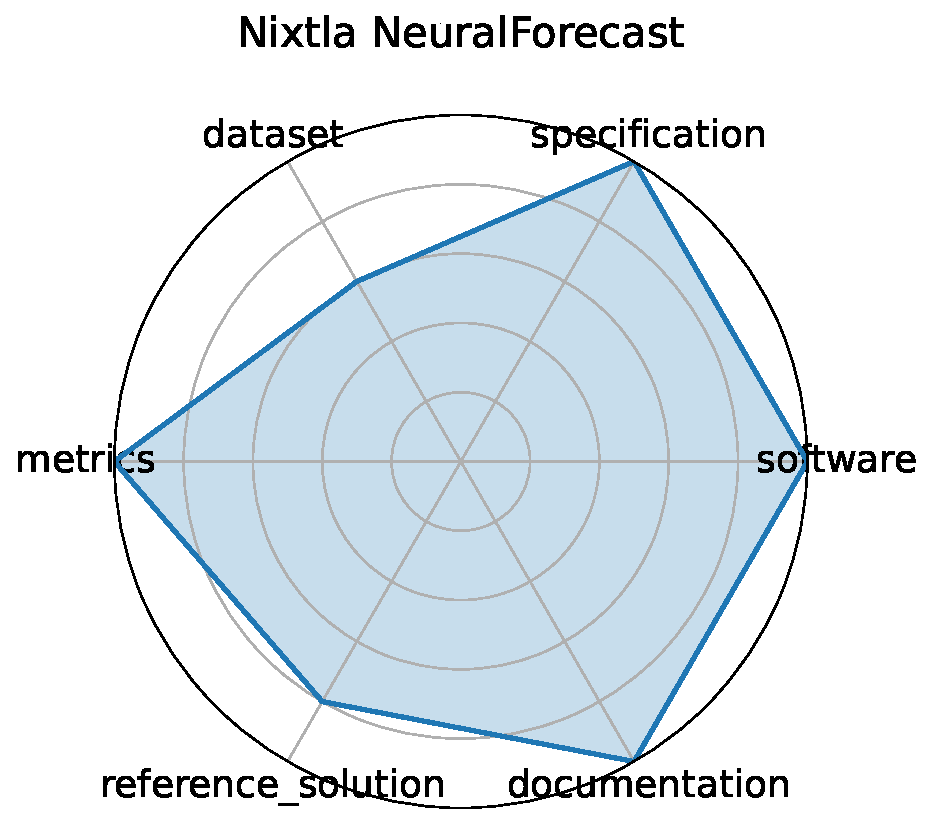
\includegraphics[width=0.2\textwidth]{nixtla_neuralforecast_radar.pdf}
}}
\clearpage